% !TeX root = ../../thesis.tex
\chapter{Tissue growth modeling}\label{ch:tissue}

\begin{shaded}
This chapter contains partial results from previously published content in \textit{Advanced Functional Materials}:\\
D. Van, B. Liang, S. Anania, M. Barzegari, B. Verlée, G. Nolens, J. Pirson, L. Geris, F. Lambert, ``3D-Printed Synthetic Hydroxyapatite Scaffold With In Silico Optimized Macrostructure Enhances Bone Formation In Vivo,'' \textit{Advanced Functional Materials}, vol. 32, p. 2105002, 2022.
\end{shaded}


\section{Introduction}

This chapter focuses on developing computational models of the curvature-driven tissue growth process, which can be coupled with the biodegradation model to have a hybrid model of biodegradation of biomaterials combined with the growth of neotissue around them. Such a coupled model can be useful for tuning the biodegradation rate to the rate of regeneration of new tissue. Similar to the biodegradation model, the modeling of the tissue formation process can take advantage of the interface tracking techniques in which the neotissue surface evolves over time, representing the growth process. Neotissue growth in porous scaffolds has been shown to be depending on the local mean curvature of the interface between the neotissue and the surrounding void space \cite{Bidan2012, Bidan2012a, Rumpler2008}. The commonly-used interface tracking techniques provide an efficient way to formulate curvature-driven problems. 

Numerical tracking of interface movement has been widely used for certain modeling applications in science and engineering for multi-material and multiphase problems such as solidification, melting, corrosion, and grain growth to name a few \cite{Sun2007}. The most popular Eulerian methodologies in this regard are the level-set \cite{Osher1988,Andrew2000,RonaldFedkiw2002}, volume-of-fluid (VOF) \cite{Rider1998}, and phase-field methods \cite{Boettinger2002,Bellemans2017}. 


The basic idea of the level-set method is to employ the Hamilton-Jacobi (HJ) algorithm for solving the general interface advection equation. The independent variable in the level-set method is a signed distance function called the level-set function $\psi$ \cite{RonaldFedkiw2002}. The level-set function should be re-initialized as the interface evolves, which is the reason behind an inadvertent mass loss, one of the most prominent shortcomings of the level-set method. Although the VOF method is not vulnerable to the mass loss issue, calculating the interface curvature is difficult from the volume fraction \cite{Sun2007}, making it less efficient to be used for curvature-driven problems. 

To overcome these challenges, diffuse interface methods \cite{Anderson1998} have gained attension in recent decades, among which the phase-field method has shown potential for solving complex moving interface problems. Contrary to the level-set method, the interface is considered a smooth transition between phases, which usually has a finite width in diffuse interface methods. In the phase-field method, a non-conserved (or conserved) order parameter $\phi$ is defined such that $\phi=1$ in one bulk phase and $\phi=-1$ in the other. Then, the smooth transition between these two phases ($-1<\phi<1$) is marked as the interface. One of the advantages of the phase-field method is that the derived equation can be solved over the entire desired domain without considering the location of the interface. Moreover, although the curvature and interface normal vectors are not formulated explicitly, the phase-field method is suitable for problems in which the evolution of the interface depends on the local curvature or a field acting normal to the interface \cite{Sun2007}. The phase-field method keeps a constant thickness for the smooth transition region normal to the interface, and as a result, no re-initialization as for the level-set method is needed.



The phase-field method has been already proved to be an efficient interface tracking technique for various problems in micro/meso scales such as solidification \cite{Karma1998,Boettinger2002}, microstructural evolution \cite{Chen2002}, grain growth \cite{Chen1994}, crack propagation \cite{Henry2004,Spatschek2011}, electromigration \cite{Bhate2000}, and extractive metallurgy \cite{Bellemans2017}. However, it has been used recently for dealing with problems described in macro level, such as corrosion \cite{Mai2016,Lin2019,Imanian2018,Lin2020,Ansari2018,Tsuyuki2018,Chadwick2018} and cell/tissue growth \cite{Jeong2017,Lee2019}. In this work, a phase-field model of the tissue growth process was developed to describe the cell growth behavior on 3D surfaces as a moving-boundary problem. Additionally, a similar model was developed based on the level-set method to compare the performance and results of both interface tracking methods. Both models were implemented using the finite element method. 


\section{Deriving the model}

This section demonstrates the derivation of the phase-field and level-set equations from the general advection equation, showing the similarities and differences of these interface tracking techniques for moving boundary problems.

\subsection{General equation of interface motion}

The general interface advection equation for an Eulerian description of interface movement can be written as \cite{Sun2007}:

\begin{equation} \label{eq:general_advec}
\frac{\partial \phi}{\partial t}+\boldsymbol{u} \cdot \nabla \phi=0,
\end{equation}
where $\phi$ is the phase field and $\boldsymbol{u}$ is the interface velocity. The velocity $\boldsymbol{u}$ can be divided into normal ($u_{\mathrm{n}}$) and external velocity components ($\boldsymbol{u}_{\mathrm{e}}$):
\begin{equation} \label{eq:two_comp_advect}
\boldsymbol{u}=u_{\mathrm{n}} \boldsymbol{n}+\boldsymbol{u}_{\mathrm{e}},
\end{equation}
in which $\boldsymbol{n}=\nabla \phi /|\nabla \phi|$ is the unit vector normal to the interface. So, Eq. \ref{eq:general_advec} can be rewritten as:
\begin{equation}
\frac{\partial \phi}{\partial t}+u_{\mathrm{n}}|\nabla \phi|+\boldsymbol{u}_{\mathrm{e}} \cdot \nabla \phi=0.
\end{equation}

The normal velocity can be decomposed into more components to take into account the effect of interface curvature ($\kappa$) such that the terms are independent and proportional to the curvature, respectively:
\begin{equation}
u_{\mathrm{n}} = a - b \kappa,
\end{equation}
where the coefficients $a$ and $b$ have units of $\mathrm{m}/\mathrm{s}$ and $\mathrm{m}^2/\mathrm{s}$. Substituting this into Eq. \ref{eq:two_comp_advect}  yields the final form of the interface motion equation:
\begin{equation} \label{eq:advect_kappa}
\frac{\partial \phi}{\partial t}+a|\nabla \phi|+\boldsymbol{u}_{\mathrm{e}} \cdot \nabla \phi=b \kappa|\nabla \phi|.
\end{equation}


\subsection{Phase-field formulation}

To further proceed with the phase-field formulation, a proper kernel should be selected for the phase field variable, which can be done based on Beckermann et al. \cite{Beckermann1999}:
\begin{equation} \label{eq:kernel}
\phi=-\tanh \left(\frac{n}{\sqrt{2} W}\right),
\end{equation}
in which $W$ is the thickness of the transition profile ($\phi$ varies from $-0.9$ to $+0.9$ in a narrow layer with the width of $3 \sqrt{2} W$), and $n$ is the coordinate normal to the interface. The curvature can be written as a function of the phase field variable:
\begin{equation}  \label{eq:curvature}
\kappa=\nabla \cdot \boldsymbol{n}=\nabla \cdot\left(\frac{\nabla \phi}{|\nabla \phi|}\right)=\frac{1}{|\nabla \phi|}\left[\nabla^{2} \phi-\frac{(\nabla \phi \cdot \nabla)|\nabla \phi|}{|\nabla \phi|}\right].
\end{equation}

Using the defined kernel, the terms in Eq. \ref{eq:curvature} can be expressed as:
\begin{equation} \label{eq:normal_terms}
|\nabla \phi|=-\frac{\partial \phi}{\partial n}=\frac{1-\phi^{2}}{\sqrt{2} W} \quad \text { and } \quad \frac{(\nabla \phi \cdot \nabla)|\nabla \phi|}{|\nabla \phi|}=\frac{\partial^{2} \phi}{\partial n^{2}}=-\frac{\phi\left(1-\phi^{2}\right)}{W^{2}}.
\end{equation}

Substituting Eq. \ref{eq:normal_terms} into Eq. \ref{eq:curvature} yields to the following definition of interface curvature: 
\begin{equation}
\kappa=\frac{1}{|\nabla \phi|}\left[\nabla^{2} \phi+\frac{\phi\left(1-\phi^{2}\right)}{W^{2}}\right],
\end{equation}
which subsequently changes Eq. \ref{eq:advect_kappa} into:
\begin{equation} \label{eq:phase_field_semifnal}
\frac{\partial \phi}{\partial t}+a|\nabla \phi|+\boldsymbol{u}_{\mathrm{e}} \cdot \nabla \phi=b\left[\nabla^{2} \phi+\frac{\phi\left(1-\phi^{2}\right)}{W^{2}}\right].
\end{equation}

Eq. \ref{eq:phase_field_semifnal} is the derived form of the phase-field equation for tracking an evolving interface, containing terms corresponding to normal interface motion, advection by an external field, and curvature-driven movement. The term $|\nabla \phi|$ in Eq. \ref{eq:phase_field_semifnal} can be replaced by its definition in Eq. \ref{eq:normal_terms} to form another version of the equation:

\begin{equation} \label{eq:phase_field_final}
\frac{\partial \phi}{\partial t}+a \frac{1-\phi^{2}}{\sqrt{2} W}+\boldsymbol{u}_{\mathrm{e}} \cdot \nabla \phi=b\left[\nabla^{2} \phi+\frac{\phi\left(1-\phi^{2}\right)}{W^{2}}\right],
\end{equation}
which is an easier version to be implemented using numerical methods. The unique term on the right-hand side of Eq. \ref{eq:phase_field_final} is a characteristic of the phase-field method.

\subsection{Level-set formulation}

From the mathematical perspective, the level-set equation has a direct connection to the phase-field equation and can be derived by replacing the phase field variable with a sign distance function. To this end, Eq. \ref{eq:advect_kappa} can be rewritten to be a level-set equation:
\begin{equation} \label{eq:ls_general}
\frac{\partial \psi}{\partial t}+a|\nabla \psi|+\boldsymbol{u}_{\mathrm{e}} \cdot \nabla \psi=b \kappa|\nabla \psi|,
\end{equation}
with $\psi$ being a sign distance function that descibes the distance of each point of the computational domain to the interface. This implies that the zero iso-contour of the level-set function defines the interface.

\section{Dimensionless forms for various cases}

\subsection{Stationary interface}

A stationary interface, where there is no interface motion ($a=0$ and $\boldsymbol{u}_{\mathrm{e}}=0$), is a primary problem in examining the formulation and select proper grid spacing parameters. For a 1-D case, Eq. \ref{eq:phase_field_final} can be simplified as:
\begin{equation} \label{eq:stationary_general}
\frac{\partial \phi}{\partial t}=b\left(\frac{\partial^{2} \phi}{\partial x^{2}}+\frac{\phi\left(1-\phi^{2}\right)}{w^{2}}\right).
\end{equation}

To scale this equation, the following dimensionless variables can be defined:
\begin{equation} \label{eq:dimenless_variables}
x^\prime = \frac{x}{x_c} \quad \text{and} \quad t^\prime = \frac{t}{t_c}.
\end{equation}

So, Eq. \ref{eq:stationary_general} can be rewritten using these new variables:
\begin{equation} 
\frac{1}{t_{c}} \frac{\partial \phi}{\partial t^{\prime}}=\frac{b}{x_{c}^{2}} \frac{\partial^{2} \phi}{\partial x^{2}}+\frac{b}{w^{2}} f(\phi).
\end{equation}

Defining $x_c = w$ and $t_c=w^2/b$ leads to the following dimensionless form of Eq. \ref{eq:stationary_general}:

\begin{equation} \label{eq:stationary_dimenless}
\frac{\partial \phi}{\partial t^{\prime}}=\frac{\partial^{2} \phi}{\partial x^{\prime 2}}+\phi\left(1-\phi^{2}\right).
\end{equation}

Numerical results for Eq. \ref{eq:stationary_dimenless} is depicted in Fig.  \ref{fig:fig:pf_ls}, and the phase field profile is compared with the level-set distance function profile. An appropriate value for grid spacing and the layer width should be selected such that $0.25 w < \Delta x^\prime < 0.5 w $. Additionally, the selected value of $w$ should satisfy $w < R/4.2$, in which $R$ is the local radius of curvature \cite{Sun2007}.

\begin{figure}
\medskip
\centering
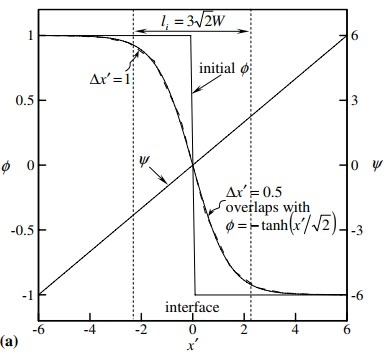
\includegraphics[width=0.7\textwidth]{pf_ls.jpg}
\caption[Comparison of phase field variable and level-set function]{Comparison of phase field variable and level-set function on the interface of a stationary interface with step function like initial condition \cite{Sun2007}}
\label{fig:fig:pf_ls}
\end{figure}


\subsection{Evolution under constant normal speed}

For a problem in which the interface moves with constant velocity exclusively, Eq. \ref{eq:phase_field_final} can be simplified according to the condition of $a=\text{const.}$, $\boldsymbol{u}_{\mathrm{e}}=0$, and $b=0$ ($b$ exists in the equation as a numerical parameter for smoothing the interface and relaxation behavior of the phase-field profile):
\begin{equation}
\phi_{t}+a \frac{1-\phi^{2}}{\sqrt{2} w}=b \phi_{xx} + b\frac{f(\phi)}{w^{2}}.
\end{equation}

Defining dimensionless variables according to Eq. \ref{eq:dimenless_variables} yields to:
\begin{equation}
\frac{1}{t_c}\phi_{t^{\prime}}+\frac{a}{w} \frac{1-\phi^{2}}{\sqrt{2}}=\frac{b}{w^2} \phi_{x^{\prime}x^{\prime}} + \frac{b}{w^{2}}f(\phi),
\end{equation}
which can be reordered to:
\begin{equation}
\phi_{t^{\prime}}+\frac{1-\phi^{2}}{\sqrt{2}}=b^{\prime}\left( \phi_{x^{\prime}x^{\prime}} + f(\phi)\right),
\end{equation}
with $b^{\prime}=b/aw$. For a stable numerical implementation, $\Delta t^{\prime}/\Delta x^{\prime} < 0.1$ and $b^{\prime} < 1.2$ should met roughly \cite{Sun2007}.


\subsection{Curvature-driven interface evolution}

A curvature-driven motion, which is desired for the current study, is straightforward to formulate using the phase-field method. In this specific case, $b$ is not a numerical parameter anymore. A dimensionless form of Eq. \ref{eq:phase_field_final} can be derived using a similar method for the stationary interface for a multidimensional case with $u_{\mathrm{n}}=-b\kappa$, $a=0$, and $\boldsymbol{u}_{\mathrm{e}}=0$:
\begin{equation} \label{eq:pf_curvature}
\frac{\partial \phi}{\partial t^{\prime}}=\nabla^{\prime 2} \phi+\phi\left(1-\phi^{2}\right),
\end{equation}
in which $t^{\prime}$ and $\nabla^{\prime}$ are defined similar to Eq. \ref{eq:dimenless_variables} as $t^{\prime}=t/(w^2/b)$ and $\nabla^{\prime}=\nabla/w$, respectively.

\section{Adapting the formulation for  curvature-driven tissue growth}

Due to intrinsic support of interface curvature in the phase-field and level-set methods, an \textit{in silico} model of curvature-based tissue growth can be efficiently implemented using these principles. The growth-induced changes in the neotissue topology during the culture process can be seen as a moving interface between two different domains \cite{Rumpler2008}. In this study, one domain represents the neotissue volume  ($\Omega_{\text{nt}}$), and the other one is the void ($\Omega_{\text{v}}$), which are separated by an interface ($\Gamma$) as can be seen in Fig. \ref{fig:growth_domain}.

\begin{figure}
\medskip
\centering
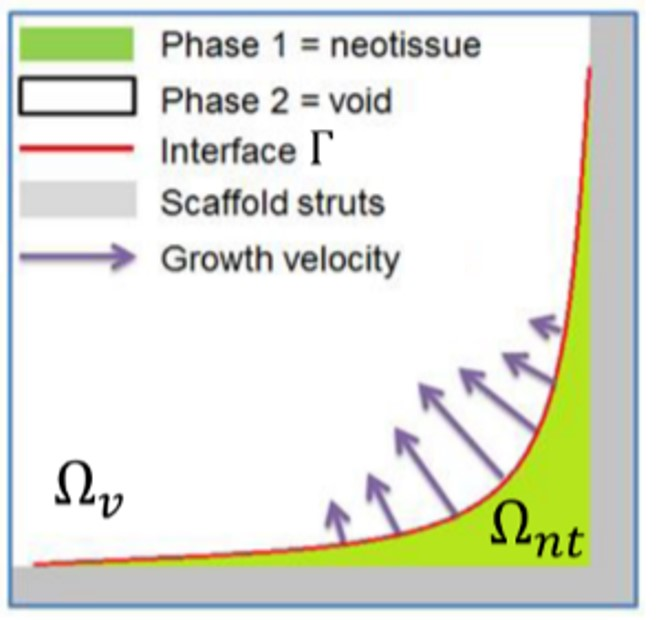
\includegraphics[width=0.5\textwidth]{growth_domain.jpg}
\caption[Schematic representation of the phase-field and level-set models for tissue growth]{Schematic representation of the phase-field and level-set models for tissue growth, in which the neotissue domain ($\Omega_{\text{nt}}$) is separated from the void domain ($\Omega_{\text{v}}$) by an interface ($\Gamma$).}
\label{fig:growth_domain}
\end{figure}

The interface $\Gamma$ evolves over time to fill the void space, having a faster growth in regions with higher curvature. Based on this definition, the phase field variable can be defined as follows to separate these domains:
\begin{equation} \label{eq:pf_domains}
\left\{\begin{array}{ll}
\phi = 1 & \text{ in } \Omega_{\text{nt}} \\
\phi = -1 & \text{ in } \Omega_{\text{v}} \\
-1 < \phi < 1 & \text{ in } \Gamma
\end{array}\right.
\end{equation}

Similarly, a level-set function can be defined such that it separates the neotissue and void domains:
\begin{equation} \label{eq:ls_domains}
\left\{\begin{array}{ll}
\psi > 0 & \text{ in } \Omega_{\text{nt}} \\
\psi < 0 & \text{ in } \Omega_{\text{v}} \\
\psi = 0 & \text{ in } \Gamma
\end{array}\right.
\end{equation}

In order to adapt Eq. \ref{eq:pf_curvature} for the curvature-driven process of neo-tissue growth, one can consider the following equation:
\begin{equation} \label{eq:pf_tissue}
\frac{\partial \phi}{\partial t^{\prime}}=\left(\nabla^{\prime 2} \phi+\phi\left(1-\phi^{2}\right)\right).H\left(\nabla^{\prime 2} \phi+\phi\left(1-\phi^{2}\right)>0\right),
\end{equation}
in which $H$ denotes a Heaviside step function. Eq. \ref{eq:pf_tissue} implies that the growth is only allowed for regions with a positive curvature (right hand side of Eqs. \ref{eq:phase_field_final} and \ref{eq:pf_curvature}).

Using the same approach, a similar level-set formulation can be obtained based on Eq. \ref{eq:ls_general} by omitting the normal velocity and curvature terms and embedding the effect of the curvature in the velocity field. Doing this yields a convection equation for the distance function:
\begin{equation} \label{eq:ls_advect}
\frac{\partial \psi}{\partial t}+\boldsymbol{u} \cdot \nabla \psi=0,
\end{equation}
in which the convection velocity field can be defined as:
\begin{equation} \label{eq:ls_veloc}
\boldsymbol{u}=\left\{\begin{array}{ll}
-\kappa \boldsymbol{n} & \text { if } \kappa>0 \\
0 & \text { if } \kappa \leq 0
\end{array}\right.
\end{equation}
with $\kappa$ being calculated similarly to Eq. \ref{eq:curvature} for a distance function $\psi$, implying that neotissue grows faster where the curvature is higher and does not grow if the curvature is negative or equal to zero \cite{Bidan2012}. The negative sign in Eq. \ref{eq:ls_veloc} is due to our definition of $\psi$, where the normal $n_\Gamma$  points toward neotissue, so growth has to be towards the opposite of the gradient of the level-set function ($ \nabla \psi$).

\section{Numerical implementation}

\subsection{Phase-field model}

The numerical solution of the phase-field equation requires dealing with the nonlinearity of the equation. Additionally, in the case of the dimensional form (Eq. \ref{eq:phase_field_final}), small coefficients of the state variable in the PDE lead to numerical difficulties. As a result, numerical implementation of the phase-field equation, especially for the spectral methods such as the finite element method, is tricky and an active field of research \cite{Shen2010,Abboud2019}. 

In the finite element method, the solution of a PDE is calculated based on a sum of a set of certain basis functions, which are commonly piecewise polynomial functions that are non-zero only on a small element. For doing this, the PDE is first written in a weak formulation, and then the weak form is projected on a discretized space (a set of elements) to be written as the summation of the basis functions. 

In this section, the numerical solution of the stationary form (Eq. \ref{eq:stationary_general}) and its corresponding considerations are elaborated as an example of employing the finite element formulation for simulating the phase-field equation. So, by assuming $b=1$ and $f(\phi)=\phi\left(1-\phi^{2}\right)$, the problem can be summarized as:
\begin{equation} \label{eq:fe_problem}
\left\{\begin{array}{ll}
\frac{\partial \phi}{\partial t}-\Delta \phi+\frac{1}{w^{2}} f(\phi)=0, & (x, t) \in \Omega \times(0, T] \\
\left.\frac{\partial \phi}{\partial n} \right|_{\partial \Omega}=0 \\
\left.u\right|_{t=0}=u_{0}
\end{array}\right.
\end{equation}
which demonstrates the PDE, the boundary condition, and the initial condition of the phase field variable where $\Omega$ is the domain of interest, $\partial \Omega$ is its boundary, and $T$ is the final time. Deriving the weak formulation of Eq. \ref{eq:fe_problem} is relatively straightforward as it can be seen as a time-dependent diffusion-reaction PDE, but the difficulty arises in choosing the numerical stability scheme for discretizing the temporal derivative and dealing with the nonlinearity of $f(\phi)$ when normally the $\frac{1}{w^{2}}$ coefficient is a small number.

Incorporating a first-order semi-explicit scheme for Eq. \ref{eq:fe_problem} yields to \cite{Abboud2019}:
\begin{equation} \label{eq:semi-implicit}
\frac{1}{\Delta t}\left(\phi^{n+1}-\phi^{n}, v\right)+\left(\nabla \phi^{n+1}, \nabla v\right)+\frac{1}{w^{2}}\left(f\left(\phi^{n}\right), v\right)=0, \quad \forall v \in H^{1}(\Omega),
\end{equation}
where $\Delta t$ is the time step, $(\cdot,\cdot)$ denotes the inner product, and $H^{1}(\Omega)$ is the Sobolev space of the domain $\Omega$, which is a space of functions whose derivatives are square-integrable functions in $\Omega$. The main issue with this discretization scheme is its restrictive time step condition which should satisfy \cite{Shen2010}:
\begin{equation}
\Delta t < \frac{2w^2}{L},
\end{equation}
where $L$ is a limit related to the non-linear part:
\begin{equation}
\max \left|f^{\prime}(\phi)\right| \leq L.
\end{equation}

Obviously, since $\Delta t \sim w^2$, a very small time step is required to achieve stability in this scheme. 

Taking advantage of a fully implicit scheme improves the stability because it will be unconditionally stable, but it results in an equation that is difficult to implement as it needs to solve a fixed point problem at each time step. For example, a modified second-order implicit Crank-Nicolson scheme for Eq. \ref{eq:fe_problem} can be written as \cite{Abboud2019,Elliott1989}:
\begin{equation}
\left(\frac{\phi^{n+1}-\phi^{n}}{\Delta t}, v\right)+\left(\nabla \frac{\phi^{n+1}+\phi^{n}}{2}, \nabla v\right)+\frac{1}{w^{2}}\left(\tilde{f}\left(\phi^{n+1}, \phi^{n}\right), v\right)=0, \quad \forall v \in H^{1},
\end{equation}
where:
\begin{equation}
\tilde{f}(u, v)=\left\{\begin{array}{ll}
\frac{F(u)-F(v)}{u-v} & \text { if } u \neq v \\
f(u) & \text { if } u=v
\end{array}\right.
\end{equation}
in which $F$ is the potential term ($f(\phi)=F^{\prime}(\phi)$).

An alternative can be deriving a stabilized semi-implicit scheme by adding a stabilization term to Eq. \ref{eq:semi-implicit}. The first-order version of such a scheme can be written as:
\begin{equation}
\left(\frac{1}{\Delta t}+\frac{S}{w^{2}}\right)\left(\phi^{n+1}-\phi^{n}, v\right)+\left(\nabla \phi^{n+1}, \nabla v\right)+\frac{1}{w^{2}}\left(f\left(\phi^{n}\right), v\right)=0, \quad \forall v \in H^{1}(\Omega),
\end{equation}
which is unconditionally stable for any $S \geq \frac{L}{2}$ \cite{Shen2010}.


\subsection{Level-set model}

The derived level-set PDE (Eq. \ref{eq:ls_advect}) is an advection equation, which can be implemented numerically using the finite element method, in which the temporal term is discretized by the backward Euler method, and the advection term can be treated with the method of characteristics. 

A key parameter of the developed model is the local growth velocity of the neotissue. In the current implementation, the velocity was dependent on the interface's local mean curvature as shown in \cite{Bidan2012a,Guyot2014}. In order to match the growth velocity to experimental data, a coefficient can be added to the derived interface convection velocity (Eq. \ref{eq:ls_veloc}):
\begin{equation} \label{eq:ls_veloc2}
\boldsymbol{u}=\left\{\begin{array}{ll}
-\kappa A \boldsymbol{n} & \text { if } \kappa>0 \\
0 & \text { if } \kappa \leq 0
\end{array}\right.
\end{equation}

The model calibration performed by Guyot et al. \cite{Guyot2014} was for a culture condition on titanium scaffolds in a bioreactor setting, estimating parameter $A$ to be $4\times10^{-14} \text{m}^2/\text{s}$, obtained using trial and error from the experimental data on low flow rate tests \cite{Papantoniou2014}.
More dedicated calibration experiments were performed on prismatic structures, demonstrating a considerably slower growth on the CaP scaffolds, nevertheless confirming the curvature-based nature of tissue growth \cite{Hede2021}.

In practical implementations, the distance function is not differentiable at every location of the domain due to discontinuities in the gradients, so one can consider taking advantage of artificial diffusion terms to overcome this issue, leading to the following equations for the normal vector and curvature calculation:
\begin{equation}
\boldsymbol{n}=\frac{\nabla \varphi}{|\nabla \varphi|}+\varepsilon \Delta \boldsymbol{n}
\end{equation}
\begin{equation}
\kappa=\nabla \cdot \boldsymbol{n}+\varepsilon \Delta \kappa,
\end{equation}
in which $\varepsilon$ denotes the numerical diffusion coefficient.


\section{Simulation setup}

Numerical simulations of neotissue formation on various shapes (scaffolds) were carried out using the developed phase-field and level-set models to compare their performance. In 2D, two shapes were used, a square and a semi-circle (Fig. \ref{fig:tissue_domain_geometry}), which were simulated using both phase-field and level-set models. In 3D, the phase-field model was evaluated on a cube, while the level-set model was used to simulate the cell growth behavior on scaffolds with triply periodic minimal surface (TPMS) shapes. 

\begin{figure}
\medskip
\centering
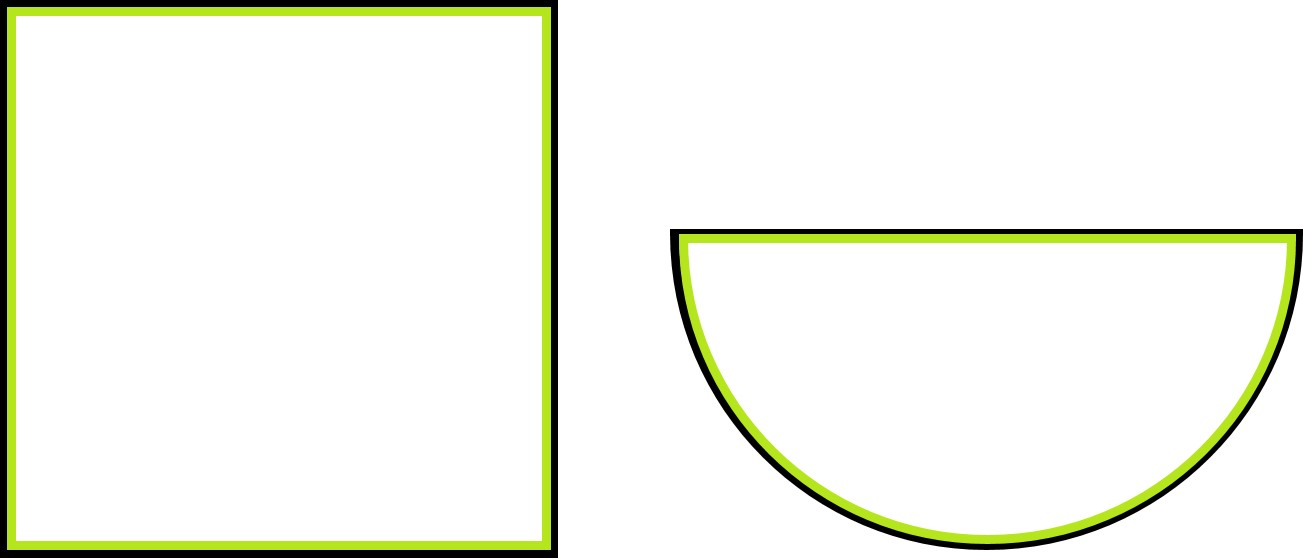
\includegraphics[width=0.6\textwidth]{domain_geometry.jpg}
\caption[Schematic representation of the simulation domains]{Schematic representation of the simulation domains}
\label{fig:tissue_domain_geometry}
\end{figure}

The initial configuration of the phase field variable and level-set distance function corresponds to a homogenous single cell layer over the scaffold struts with a thickness equal to $20 \mu m$ in a dimensional setup \cite{Darling2008}. This is depicted as the green layer in Fig. \ref{fig:tissue_domain_geometry}. For the 3D level-set model, neotissue growth was simulated for a variety of TPMS family and compared in a qualitative manner. A full quantitative prediction is not possible due to the absence of relevant validation experiments, which explains why comparisons between geometries are made over non-dimensional time. 

The derived weak forms were implemented using FreeFEM open-source PDE solver \cite{Hecht2012}. Eulerian computational mesh for each simulation was constructed by generating tetrahedral elements using the internal mesh generator of FreeFEM, called BAMG. To decrease run time and increase the performance of the simulation, the mesh was partitioned using  METIS \cite{METIS1998} and HPDDM preconditioner \cite{Jolivet2013}, available in FreeFEM and PETSc toolkit \cite{petsc}. Moreover, the efficiency was boosted by using the HYPRE BoomerAMG preconditioner \cite{Falgout2002} and the GMRES iterative solver \cite{Saad1986} of the PETSc toolkit.


\section{Results and Discussion}

In the current study, various 2D and 3D cases for the simulation of curvature-based neotissue formation were prepared and separately simulated using the phase-field and level-set models. The cases were a square and a semi-circle for 2D simulations, on the circumstance of which the cells were seeded to initiate the tissue growth. Similarly, a 3D cube was considered for evaluating the performance of the phase-field implementation in 3D. Additionally, the level-set model was used to simulate cell proliferation on TMPS scaffolds with quantitative measurements being carried out for the percentage and filling rate of generation of neotissue.

The results of tissue growth model simulations can be visualized by depicting the +1 part of the phase field variable (Eq. \ref{eq:pf_domains}) and the positive part of the level-set function (Eq. \ref{eq:ls_domains}). Fig. \ref{fig:tissue_simulation_square} demonstrates such a visualization for the phase-field and level-set simulations performed on the square domain. Cells were seeded on the circumstance of the square, and the formation of neotissue was modeled using the evolution of the phase field variable and level-set function. The light gray region in these figures shows the +1 part of the phase field variable and the positive part of the level-set function.

\begin{figure}
\medskip
\centering
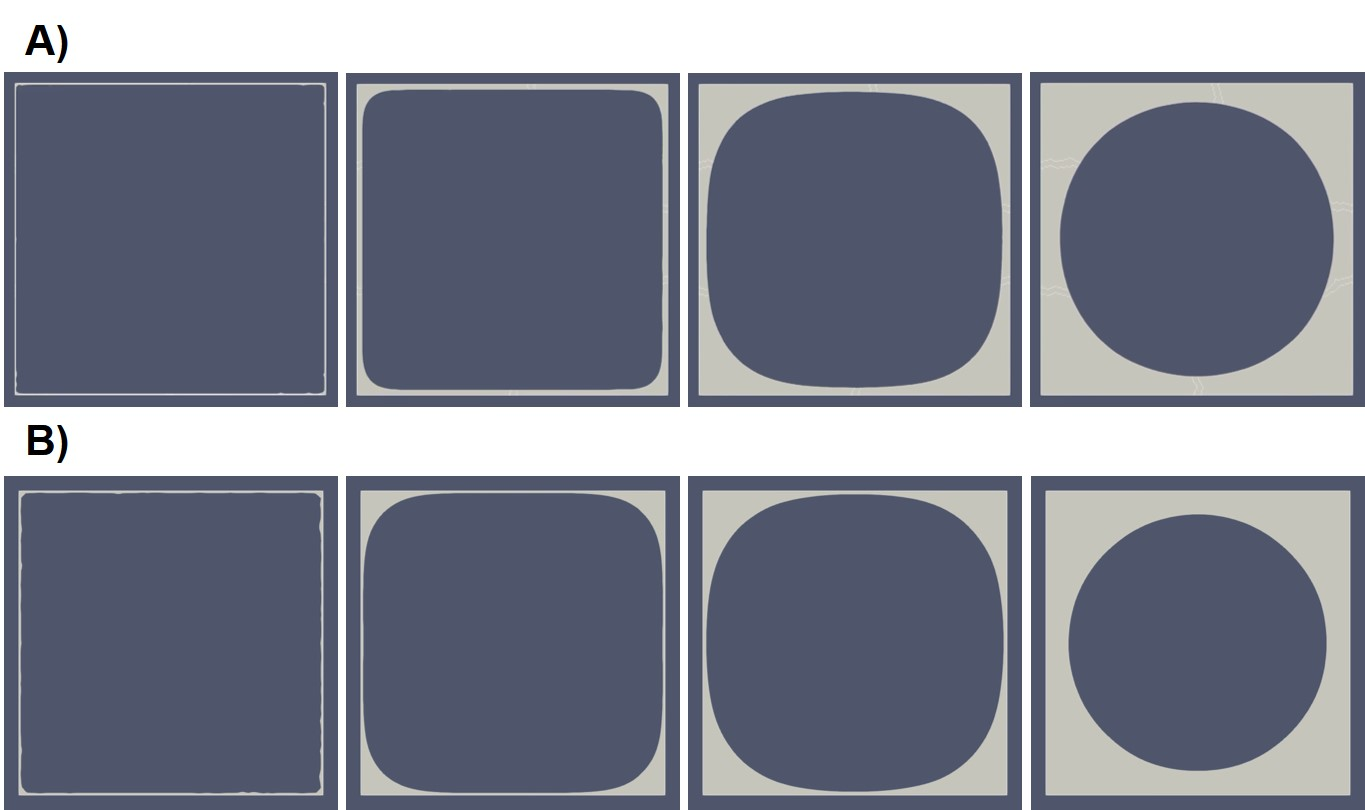
\includegraphics[width=\textwidth]{simulation_square.jpg}
\caption[Simulation result of tissue growth in the square domain]{Simulation result of the phase-field (A) and level-set (B) models for tissue growth in the square domain. The light gray region shows the +1 part of the phase field variable and the positive part of the distance function for the phase-field (A) and level-set (B) models, respectively. The evolution occurs from left to right.}
\label{fig:tissue_simulation_square}
\end{figure}

As shown in Fig. \ref{fig:tissue_simulation_square}, a qualitative comparison of the evolution of the formed tissue interface between the phase-field and level-set models indicates that they capture the curvature-driven growth similarly. It seems that the level-set model resulted in more sharp interfaces, in which the surfaces without curvature do not move at all in absence of curvature. But, in the phase-field predictions, the surfaces not having any curvature slightly move. This can be seen by comparing the growth pattern on the top edge of the square, where it starts to grow only in the fourth row in Fig. \ref{fig:tissue_simulation_square} for the level-set results, while a minor move can be seen in the phase-field predictions. This slightly different behavior can be related to the implementation details, such as the lack of a proper Heaviside function in FreeFEM that the phase-field model depends on. Another possible reason for this difference can be the visualization aspect since the transition region of the phase field variable representing the surface is thicker in the phase-field model in comparison to the zero iso-contour of the level-set function. As a result, the evolution can be artificially plotted in the visualization software, which was ParaView in this case. This effect can be investigated further by refining the mesh to minimize artificial evolution. 

A similar visualization is depicted in Fig. \ref{fig:tissue_simulation_circle} for the neotissue formation on the semi-circle domain. Results show that the phase-field and level-set models have good agreement on the way they treat the curvature-based tissue growth. As seen in the figure, both models show identical predictions on the surface with curvature (the curvy edge of the semi-circle). However, the small difference observed for the square case can also be seen here on the top surface, where the neotissue grows slightly faster in the phase-field model.

\begin{figure}
\medskip
\centering
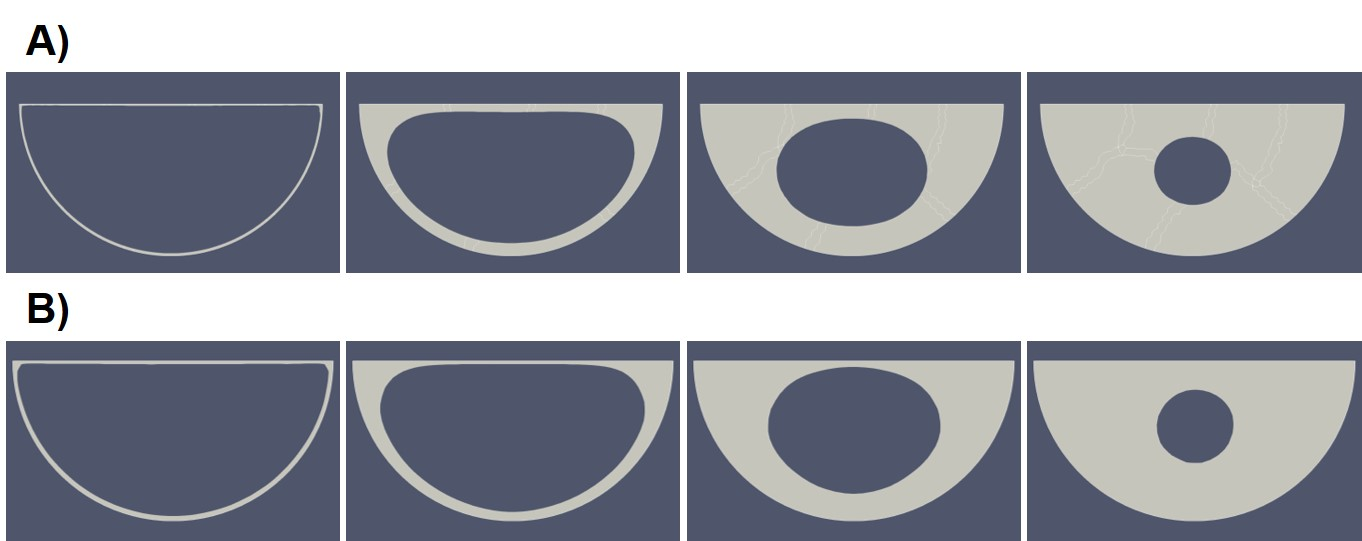
\includegraphics[width=\textwidth]{simulation_circle.jpg}
\caption[Simulation result of tissue growth in the semi-circle domain]{Simulation result of the phase-field (A) and the level-set (B) models for tissue growth in the semi-circle domain. The evolution occurs from left to right.}
\label{fig:tissue_simulation_circle}
\end{figure}

Fig. \ref{fig:tissue_pf_circle_field} shows the evolution of the phase field variable corresponding to the results depicted in Fig. \ref{fig:tissue_simulation_circle}-A, demonstrating how the diffuse interface model works. In this figure, the concept of the diffusive interface can be observed, where a narrow region between the two phases (the neotissue and the void space in this case) is formed and moves over time. This visualization demonstrates the internal mechanism of the phase-field model, in which the narrow region is kept at a fixed length (defined by the kernel in Eq. \ref{eq:kernel} for a length of $3 \sqrt{2} W$) and gets advected over time by the phase-field equation (Eq. \ref{eq:phase_field_final}). In contrast, in the level-set formalism, the interface is not tracked as a fixed length region, and instead, the zero iso-contour of a signed distance function is the interface between the phases. The signed distance function maps each node of the whole space (the desired computational domain) into the distance to the interface, and as a result, the change in the function determines the movement of the interface.


\begin{figure}
\medskip
\centering
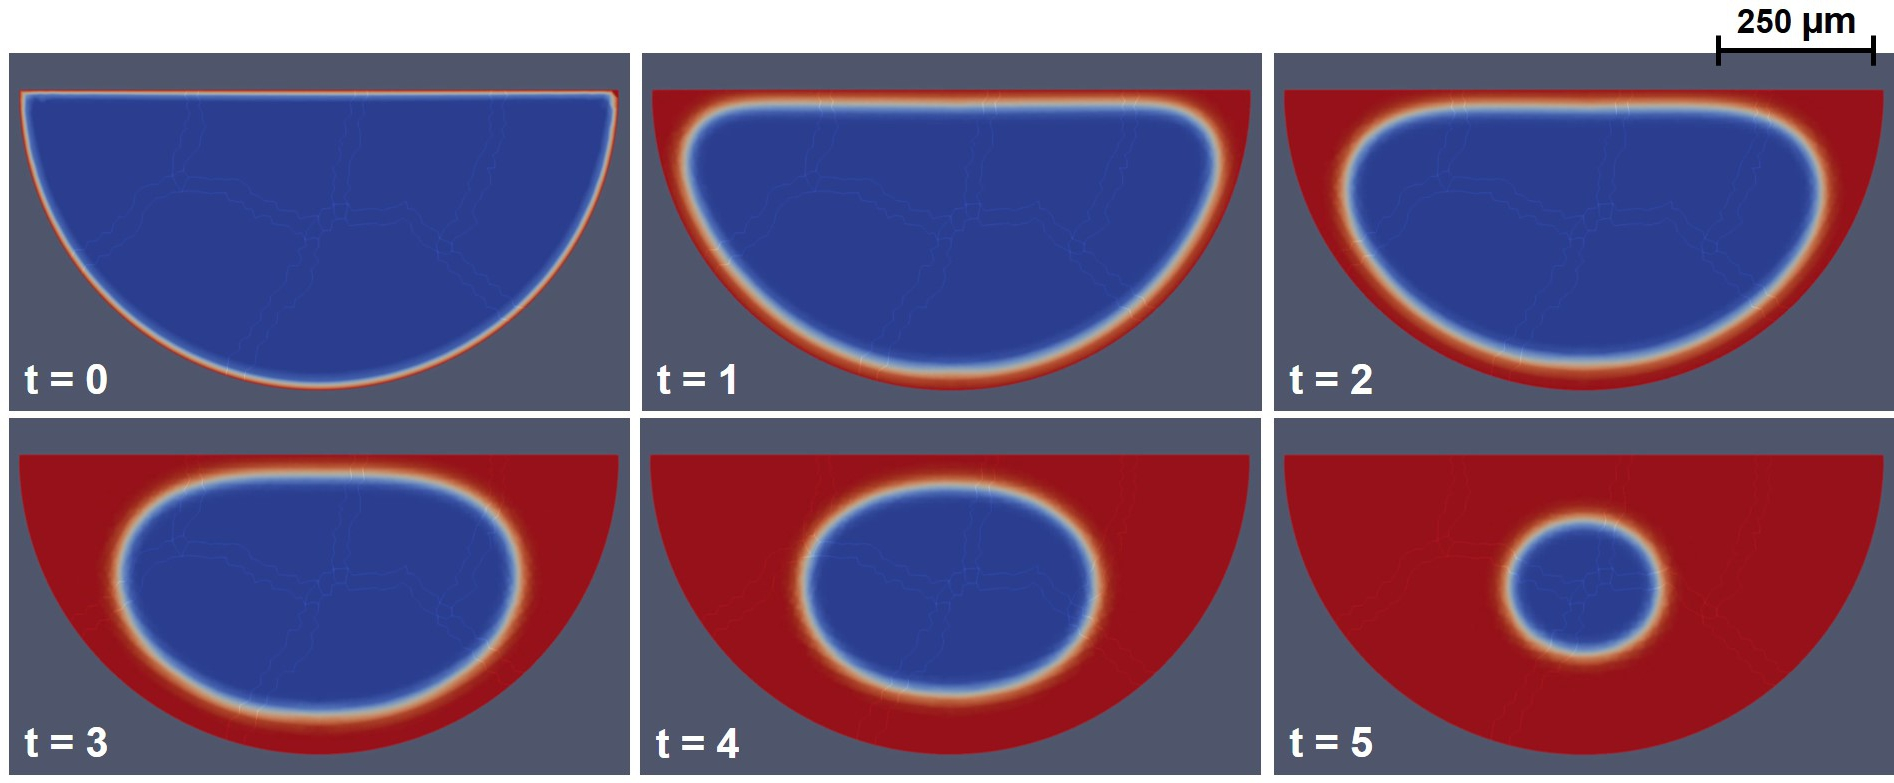
\includegraphics[width=\textwidth]{pf_circle_field.jpg}
\caption[Visualization of the evolution of phase field variable in the semi-circle domain]{Visualization of the evolution of phase field variable in the semi-circle domain. The evolution is depicted over time, occurring from top to bottom and from left to right in each row. The red, blue, and white show the +1 region, -1 region, and the transient phase representing the interface, respectively.}
\label{fig:tissue_pf_circle_field}
\end{figure}

Similar results are obtained in 3D, where the cells are seeded on the circumstance of a cuboid. Fig. \ref{fig:tissue_pf_3d} shows the simulation results of this 3D case, in which the evolution of the phase field variable is converted to a bulk of the formed neotissue. As can be seen in this figure, the phase-field model performs well in 3D, showing a similar growth behavior to the 2D model. The mesh in the 3D case is relatively coarse, but the captured behavior of tissue growth by the phase-field model seems to be more acceptable than in the 2D case. This claim can be observed on the top and bottom surfaces of the cube, where the interface doesn't move until a curvature is created in those regions, a behavior that was captured better by the level-set model in the 2D cases. 

\begin{figure}
\medskip
\centering
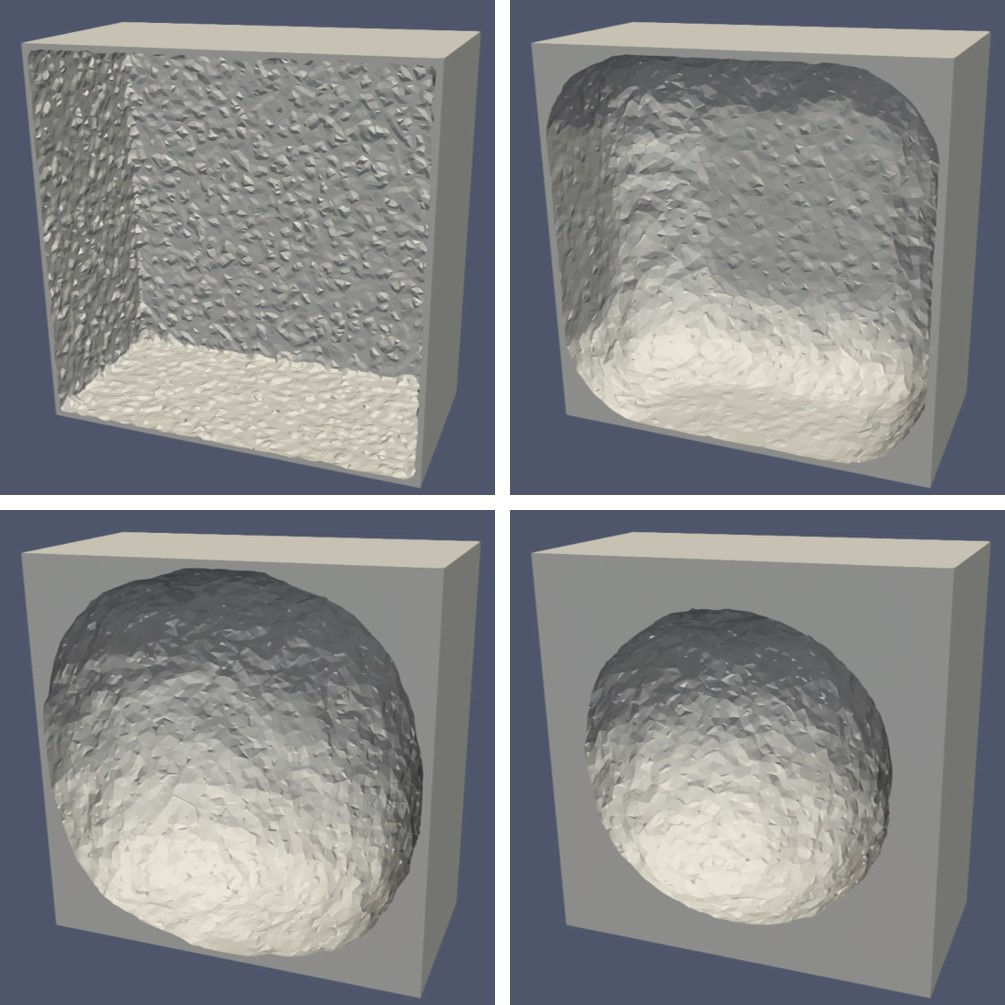
\includegraphics[width=0.7\textwidth]{pf_3d.jpg}
\caption[Simulation result of the phase-field model for tissue growth in the 3D cube domain]{Simulation result of the phase-field model for tissue growth in the 3D cube domain, in which the +1 regions of the phase field variable are visualized to show the formation of neotissue.}
\label{fig:tissue_pf_3d}
\end{figure}

Fig. \ref{fig:tissue_ls_tpms} depicts various simulation results of the netissue formation in gyroid-TPMS scaffolds, demonstrating an example of the final application of these models in action. The reason for choosing gyroid-TPMS scaffolds is their promising performance for neotissue formation due to their favourable local curvature. Various geometries for investigating the pore size and wall thickness were evaluated in order to obtain the combination leading to optimal neotissue growth. Pore size was varied between $700  \mu m$ and $1.3 mm $, and wall thickness was varied from $200 \mu m $ to $800 \mu m$, which are ranges that take into account restrictions of the manufacturing process in terms of the smallest feature dimensions. Balancing the need for swift neotissue ingrowth (Fig. \ref{fig:tissue_ls_tpms}-B, relevant for short-term implant stability) with the volume of neotissue formed (Fig. \ref{fig:tissue_ls_tpms}-A, relevant for long-term implant stability), the combination of $700 \mu m$ pore size and $200 \mu m $ wall thickness (Fig. \ref{fig:tissue_ls_tpms}-C) seemed to be the most optimal structure.

\begin{figure}
\medskip
\centering
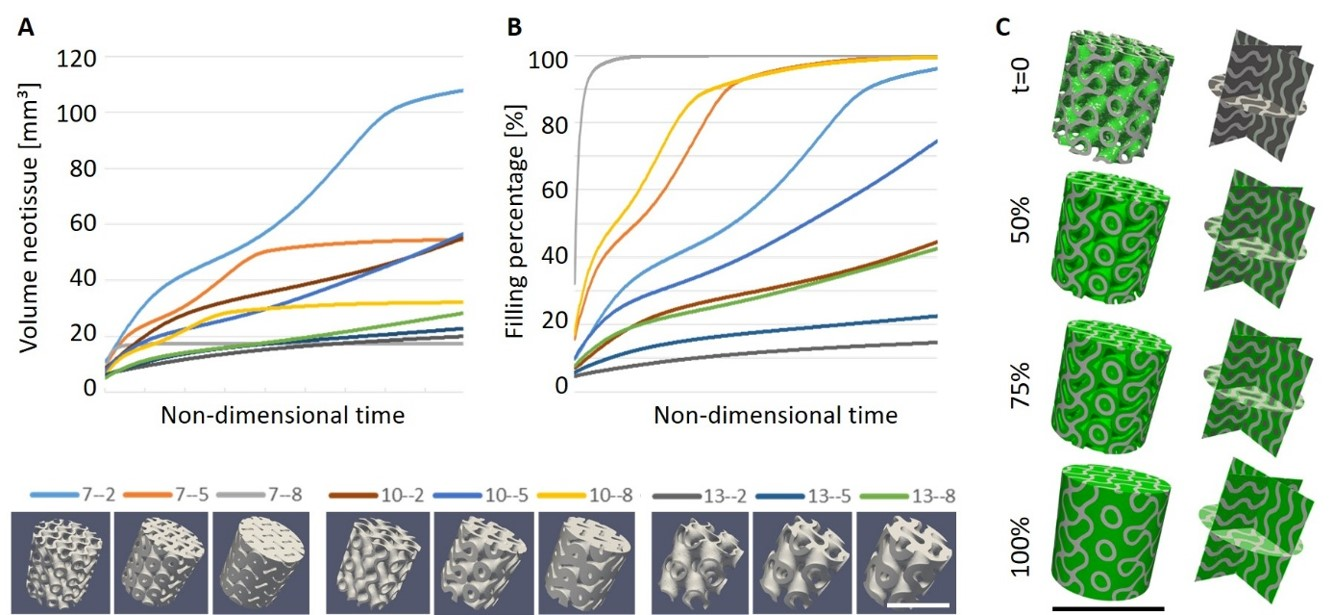
\includegraphics[width=\textwidth]{ls_tpms.jpg}
\caption[Simulation results of the level-set model for neotissue formation on TPMS scaffolds]{Neotissue formation quantified in absolute volume (A) and filling percentage (B) for cylindrical test samples (diameter 6 mm, height 6 mm). The different combinations are indicated in the legend by 2 numbers, the first of which refers to pore size (7: 700 $\mu$m, 10: 1 mm, 13: 1.3 mm), and the second refers to wall thickness (2: 200 $\mu$m; 5: 500 $\mu$m; 8: 800 $\mu$m;). (C) Side view and cross-sectional view of neotissue growth in gyroid (7-2) scaffold for different levels of filling, starting with the initial condition at t=0 (top). Scale bars: 6 mm}
\label{fig:tissue_ls_tpms}
\end{figure}

The study shown as an example above \cite{Hede2021} demonstrates the relevance of the developed tissue growth models in tissue engineering applications. \textit{In silico} modeling is widely used for tissue engineering as it offers a more exhaustive approach compared to a ``trial-and-error'' method and reduces the number of experimental tests. Optimization of scaffold structures for bone tissue engineering purposes is often corroborated by comparison with \textit{in vitro} tests \cite{Alias2017,Rubert2021} and only a small number of \textit{in vivo} studies have been reported \cite{Long2012,Luo2017,Luo2015}. However, in these \textit{in vivo} studies, optimization was first performed on mechanical properties rather than the structural elements such as local curvature underlying the used \textit{in silico} model. Having such a model developed makes it easier to investigate the structural elements of scaffolds for improved regenerative performance. Using the modeling results makes it possible to limit the number of conditions tested \textit{in vivo}.

\section{Challenges in coupling tissue growth and biodegradation models} \label{sec:tissue_challenges}

Coupling our biodegradation model \cite{Barzegari2021} with the developed tissue growth model in this chapter could have been a milestone of the current Ph.D. thesis, where the neotissue forms from the cells seeded on a biodegradable scaffold. Another interesting example could be using biodegradable porous implants in bone healing applications (similar to the model presented in Chapter \ref{ch:cup}), in which the implant degrades while new bone forms and replaces the porous implant. However, despite the effort made on tissue growth modeling, such coupling has never been accomplished successfully due to specific technical difficulties. In this section, these challenges are briefly reviewed. 

Both the biodegradation and the tissue growth models are free boundary problems, in which an interface capturing method (phase-field for the tissue growth and level-set for the biodegradation) was used to track the movement of a boundary. The moving boundary in the biodegradation model is the corrosion front, the interface between the metallic part and the surrounding environment, which can be a static electrolyte in immersion tests or circulated solutions in a perfusion setup. Various mass transfer boundary conditions are defined on this boundary \cite{Barzegari2021}, meaning that the boundary conditions are not fixed and move with the evolution of the surface. In other words, the boundary conditions of a set of equations are defined on the solution of one of the governing equations of the model (level-set equation), which is one of the challenging parts of the implementation of that model. On the other hand, the moving boundary in the tissue growth model is the surface of the formed neotissue, the interface between the neotissue and the surrounding environment in the bioreactor, which is considered as the void space since there is no neotissue in that region. Coupling these two models requires defining the moving boundary problem of tissue growth on the solution of the interface capturing of the biodegradation model. No matter of either using the same technique for both problems or using separate methods for each problem, such coupling can be quite challenging from the implementation perspective.

The second problem is related to the behavior of neotissue formation after coupling the models when the biodegradable material shrinks and a new void space appears at the back of the formed tissue. Fig. \ref{fig:tissue_coupling_challenge} shows this problem schematically. Fig. \ref{fig:tissue_coupling_challenge}-A shows an initial state of the coupled system, in which a level-set formulation is used for dividing the domain into the scaffold and medium parts (the $\psi$ function on the top) while a phase-field function divides the domain into tissue and void space (the $\phi$ function on the bottom). The positive side of the level-set function ($\psi > 0$) is not defined in the domain of the tissue growth model ($\phi=\text{NaN}$). After several time steps, the system enters a state similar to the one depicted in Fig. \ref{fig:tissue_coupling_challenge}-B, where the scaffold has shrunk to the left due to biodegradation, and the tissue has grown to the right. As can be seen in the figure, these movements cause a new area to appear between the scaffold and neotissue, in which the level-set function is negative ($\psi < 0$) and the phase field variable is one ($\phi=+1$). Since this area is part of the void space for the phase-field model, the tissue should grow in this direction as well, but this behavior doesn't have a clear definition from an implementation point of view. From a common-sense perspective, the tissue should attach to the surface of the scaffold and move with it to the left, a behavior that is quite challenging to consider in the formulation of the two coupled interface moving problems. Moreover, it is not fully clear how such behavior happens in experiments, so dedicated experiments are required to observe the actual reaction of the growing neotissue to the shrinkage of the scaffold. This behavior may be sensitive to experimental conditions such as static or perfusion setup of the medium, making the problem even more complex from the mathematical perspective.


\begin{figure}
\medskip
\centering
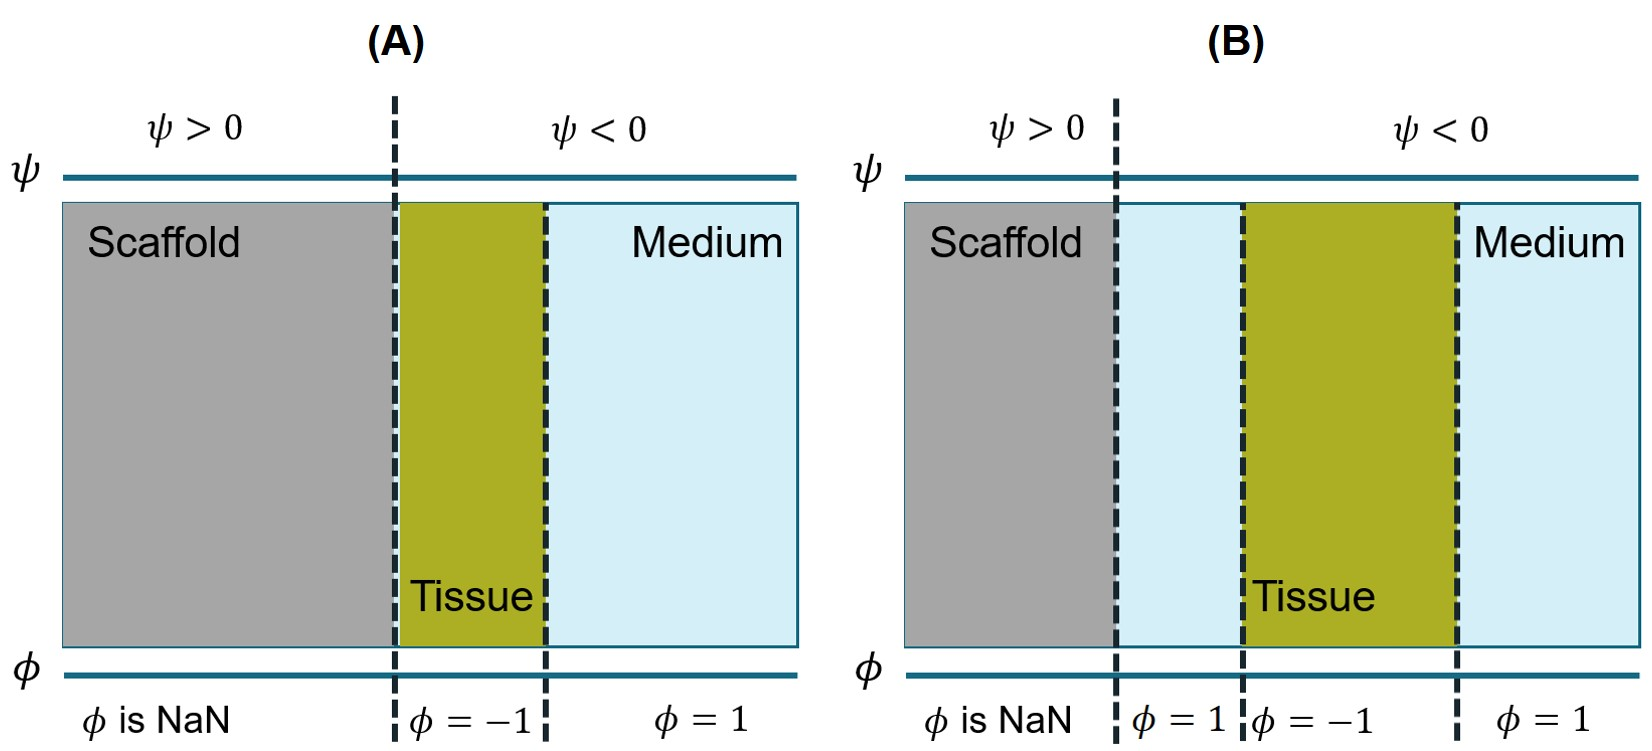
\includegraphics[width=\textwidth]{coupling_challenge.jpg}
\caption[Schematic presentation of coupled tissue growth and biodegradation models]{Schematic presentation of coupled tissue growth and biodegradation models: A) initial state of the system with level-set and phase field variables dividing the domain for the biodegradation and tissue growth models, respectively, B) the state of the system after some time steps, in which the biodegradation shrinks the scaffold to the left, the tissue grows to the right, and a new area emerges between the scaffold and the neotissue.}
\label{fig:tissue_coupling_challenge}
\end{figure}

The next challenge would be the validation of the coupled model. In addition to the necessity mentioned above for performing dedicated experiments to observe the actual behavior of tissue growth on biodegradable scaffolds, such experiments are crucial to validate the model from a quantitative point of view. Doing these experimental studies seems to be challenging and resource-demanding because both the qualitative behavior and quantitative measurements should be recorded. The qualitative behavior is crucial to observe how tissue growth reacts to the shrinkage of the material underneath, while the quantitative output of the experiments can be directly used to validate the rate of degradation and neotissue formation predicted by the coupled model. Such resource-demanding experiments were never planned as part of this Ph.D., and as a result, the coupled models could never be easily validated.


A suitable workaround for the aforementioned challenges can be coupling the biodegradation model with a simpler tissue growth model in the first place. A simpler model here implies that it does not include an interface tracking sub-model, for which the above challenges may appear in the implementation. An example of such a model is Carlier et al. work \cite{Carlier2012,Carlier2016}, in which they solved a set of taxis-diffusion-reaction PDEs describing the evolution of biochemical factors, cells, and extracellular matrices to model the healing process. Due to the lack of interface capturing, such a model is easier to integrate with the biodegradation model. A similar integration was done by Manhas et al. \cite{Manhas2016} on calcium phosphate (CaP)-based scaffolds, in which a simplified level-set shrinkage sub-model was combined with the reaction-diffusion model of the bone healing process. This approach can be more difficult to validate, but it comes with the advantage of a more straightforward implementation.


%\begin{subappendices}
%
%\section{Implementing the phase-field model using physics-informed neural networks}
%
%Dummy text for PINN model
%
%
%\begin{figure}
%\medskip
%\centering
%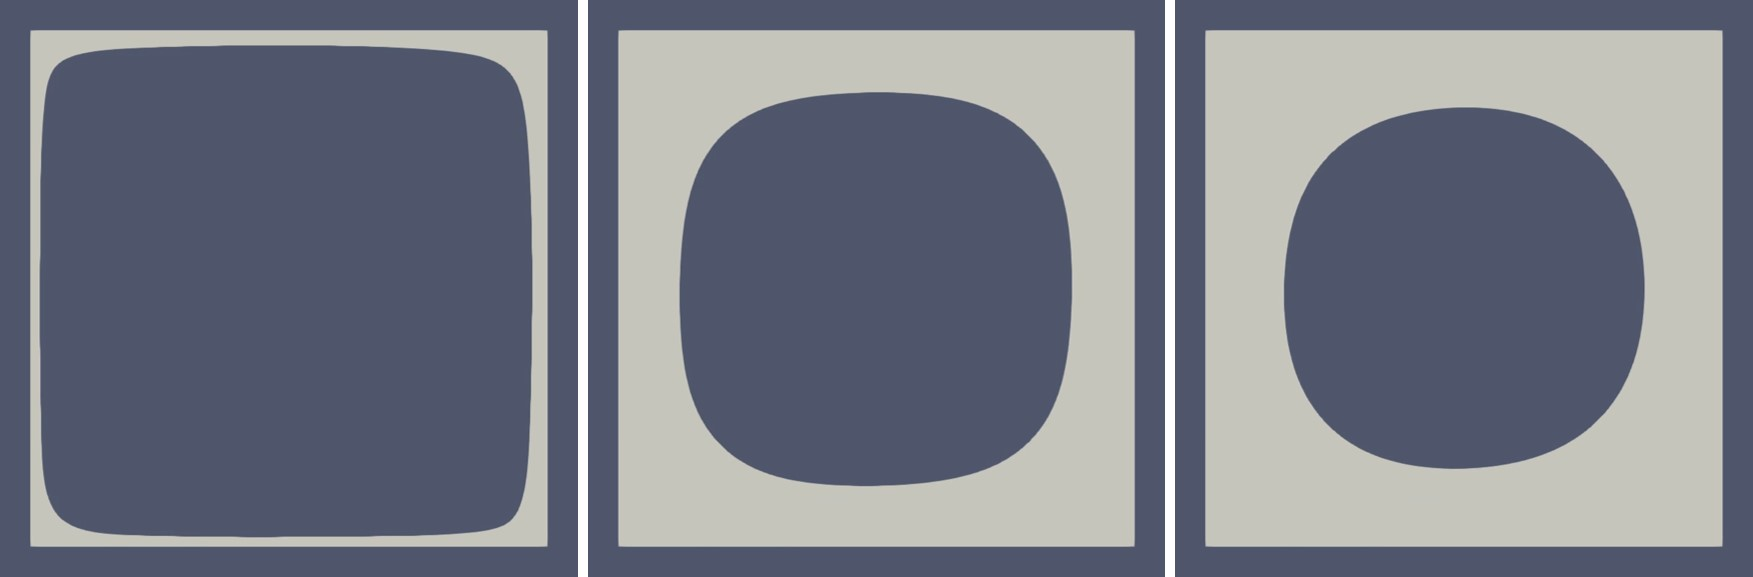
\includegraphics[width=\textwidth]{pinn_result.jpg}
%\caption[Simulation result of the PINN model for the square domain]{Simulation result of the PINN model for the square domain}
%\label{fig:tissue_pinn_result}
%\end{figure}
%
%
%
%\end{subappendices}

%%%%%%%%%%%%%%%%%%%%%%%%%%%%%%%%%%%%%%%%%%%%%%%%%%
% Keep the following \cleardoublepage at the end of this file, 
% otherwise \includeonly includes empty pages.
\cleardoublepage


